\section{Theoretical Analysis}
\label{sec:analysis}

In this section we analyse the architecture chosen for the ACDC converter circuit using an Octave theoretical model. Using the ideal diode model we were able to predict the output of the Envelope Detector and Voltage Regulator circuits.

\subsection{Envelope Detector}
Below are the values we chose for the number of coils in the transformer and for the components of the envelope detector circuit.

Due to the transition regime, that turned out to be quite lengthy, we opted to start the study of the circuit after a period of 3.8 seconds in order to have a stabilized response.
The voltage at the output of the envelope detector circuit was then plotted as follows in figure~\ref{fig:enveloped}.
\begin{figure}[h!] \centering
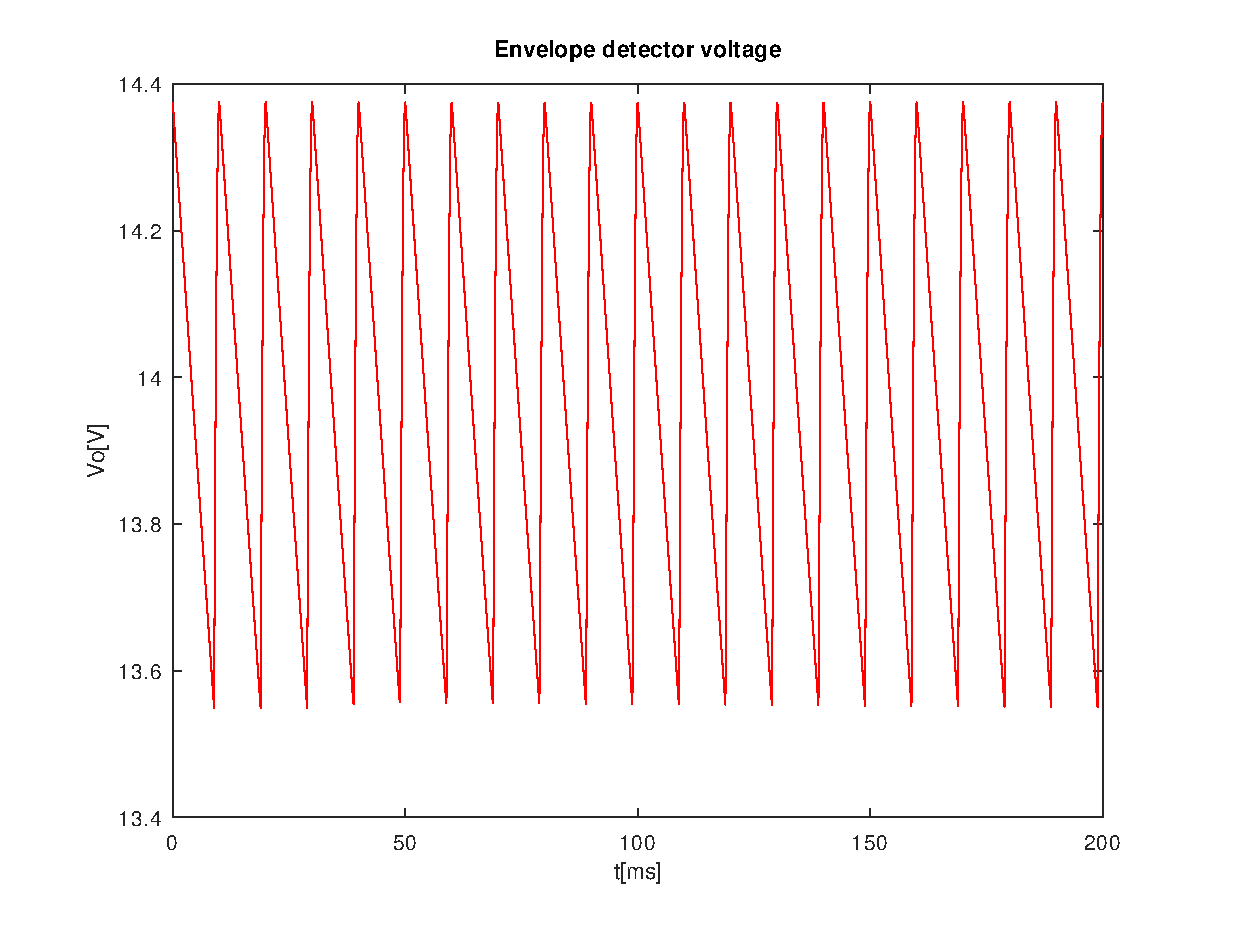
\includegraphics[width=0.9\linewidth]{Venv.eps}
\caption{Voltage envelope detector circuit output.}
\label{fig:enveloped}
\end{figure} \par
As expected, we see a positive voltage oscillating up to a maximum voltage equal to the initial 230V divided by the number of coils $\cong$ 25.2553V. Already we are close to a direct current regime, but the voltage level and the magnitude of the ripple still need to be addressed and adjusted.
\subsection{Voltage Regulator}
We used incremental analysis in order to determine the equivalent diode resistance, using the following formula.
\begin{equation}
R_d=\frac{\eta*V_T}{I_s*e^\frac{V_d}{\eta*V_T}}=~247.05;
\end{equation}
This way, we needed a resistance value much greater than the diode incremental resistance (we chose 100kOhm). The output of the regulator circuit is plotted in figures \ref{fig:reg} to \ref{fig:output} and ended up yielding a merit figure of approximately 33.6 that we hoped to replicate in the NGSpice simulation.
\begin{figure}[h!] \centering
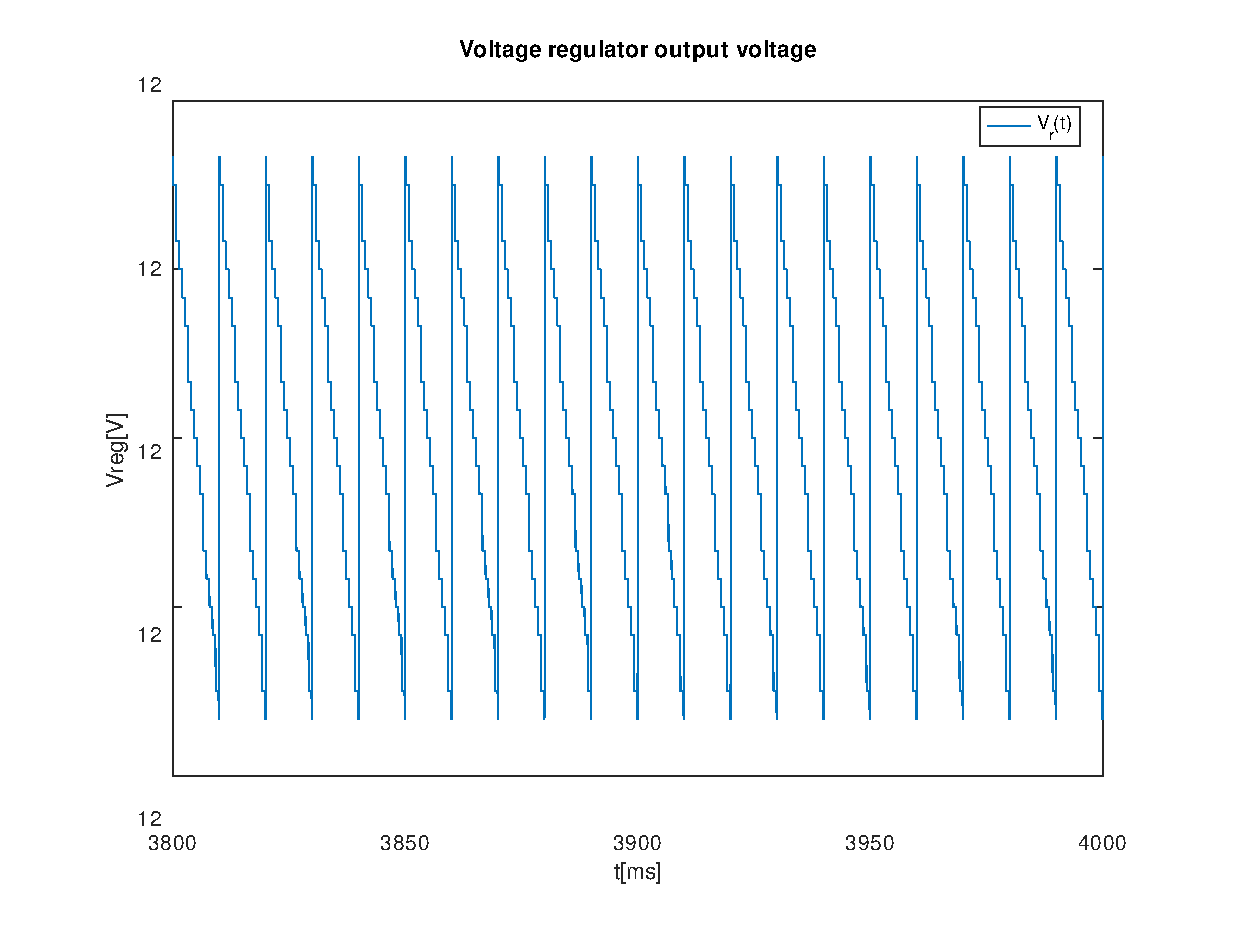
\includegraphics[width=0.9\linewidth]{Vreg.eps}
\caption{Voltage regulator circuit output.}
\label{fig:reg}
\end{figure}
\begin{figure}[h!] \centering
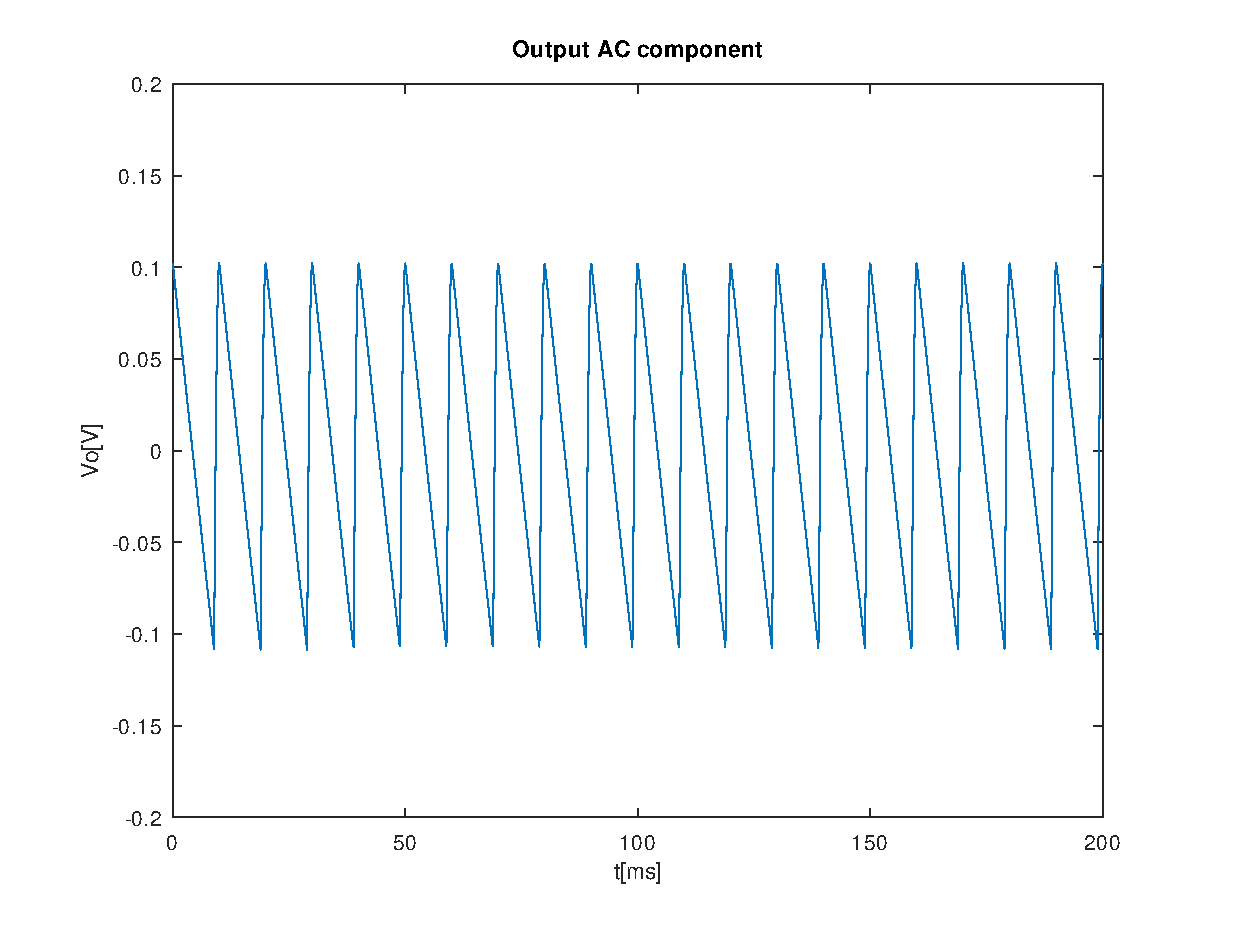
\includegraphics[width=0.9\linewidth]{deviation.eps}
\caption{Circuit output without the DC component.}
\label{fig:dc}
\end{figure}
\begin{figure}[h!] \centering
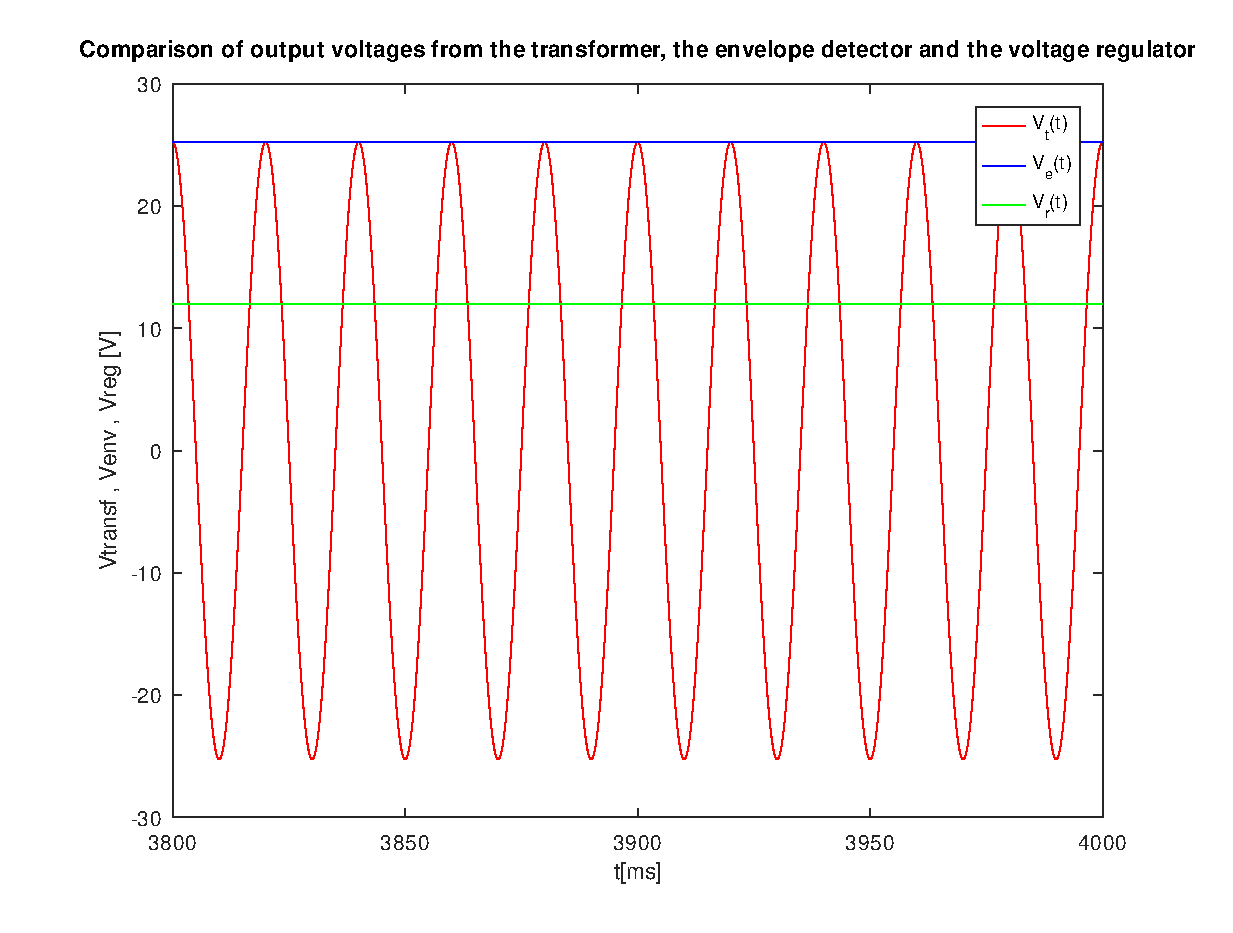
\includegraphics[width=0.9\linewidth]{comparison.eps}
\caption{Comparison between the different voltage outputs.}
\label{fig:output}
\end{figure}
\par
